\nonstopmode
\documentclass{beamer}
%\documentclass[handout]{beamer}
\includeonlylecture{intro}



\providecommand{\cpp}{C\kern-0.05em\texttt{+\kern-0.03em+} }
\providecommand{\Cpp}{\cpp}

%\usepackage{pdfpages}
\usepackage[utf8]{inputenc}
\usepackage[T1]{fontenc}
\usepackage{lmodern}
\usepackage{import}
\graphicspath{{../pics}}
%\usepackage{pgf}
%\usepackage{ctable}

\usepackage{listings}%[2000/08/23]
\usepackage{lstlangampl} % syntax file, I added some more keywords like 'display'

%\usepackage{graphicx}
%\usepackage{multicol}

%\usepackage{tikz}

\lstnewenvironment{cplus}
    {\lstset{language=c++,basicstyle=\scriptsize,frame=}}
    {}


\lstnewenvironment{cplus3}
    {\lstset{language=c++,basicstyle=\scriptsize,frame=}}
    {}


\lstnewenvironment{java}
    {\lstset{language=java,basicstyle=\scriptsize,frame=}}
    {}

\lstnewenvironment{java2}
    {\lstset{language=java,basicstyle=\scriptsize}}
    {}

\lstdefinelanguage{Haskell-custom}
{%columns=flexible,
escapeinside={--@}{@--},breaklines=true,breakatwhitespace=true%
language=Haskell,basicstyle=\color{lightblue}\ttfamily,keywordstyle=\ttfamily,%
morekeywords={class,instance,type,newtype,data,where,deriving,import},%
lineskip=-.1\baselineskip,morekeywords={concept,requires,concept_map}}

\lstnewenvironment{hask}[1][\small]{\lstset{language=Haskell-custom,%
    style=numbers,basicstyle=\color{lightblue}#1\ttfamily,keywordstyle=#1\ttfamily,%
    style=bold-keywords,style=frametb}}{}

\providecommand{\haskellinl}[2][\normalsize]{{\lstinline[language=Haskell-custom,%
basicstyle=\color{lightblue}#1\ttfamily,keywordstyle=#1\ttfamily]@#2@}}%

\providecommand{\haskinl}[2][\normalsize]{{\lstinline[language=Haskell-custom,%
basicstyle=\color{lightblue}#1\ttfamily,mathescape=true,keywordstyle=#1\ttfamily]@#2@}}%

\lstdefinestyle{markers}{rangeprefix=\{-\:\ ,%
includerangemarker=false,%
rangesuffix=\ \:-\}}%

\providecommand{\haskellinput}[3][\small]{{\lstinputlisting[language=Haskell-custom,basicstyle=\color{lightblue}#1\ttfamily,keywordstyle=#1\ttfamily,%
style=bold-keywords,style=numbers,style=frametb,style=markers,firstnumber=1,linerange={#3}]{#2}}}

\providecommand{\haskellinputnonumber}[3][\small]{{\lstinputlisting[language=Haskell-custom,basicstyle=\color{lightblue}#1\ttfamily,keywordstyle=#1\ttfamily,%
style=bold-keywords,style=frametb,xleftmargin=8pt,xrightmargin=8pt,style=markers,firstnumber=1,linerange={#3}]{#2}}}



\title[Automated Unit Test Generation]{Automated generation of Unit Tests from UML \UMLType{Activity}s using the AMPL interface for Constraint Solvers } 
%\subtitle[Airbus Model Based Engineering]{An Airbus Project on Model Based Engineering} 
\author[F. Kurth]{Felix Kurth} 
\day=13
\month=8
\year=2013
\date[\today]{\today} 

\pgfdeclareimage[height=1.2cm]{STS-logo}{STS-logo}
\logo{\pgfuseimage{STS-logo}}

\begin{document}

\begin{frame}
\titlepage
\end{frame}

\begin{frame}
\frametitle{Outline} 
\tableofcontents  
\end{frame}


\section{Motivation}

\lecture{Airbus Specific Content}{airbus}
\subsection{Model Based Engineering at Airbus}
\begin{frame}
\frametitle{Generating C-Component Code and Unit test Code from the same Model}
%\def\svgwidth{300pt} \import{../pics/}{Activity2Code+Testsfaster.pdf_tex}
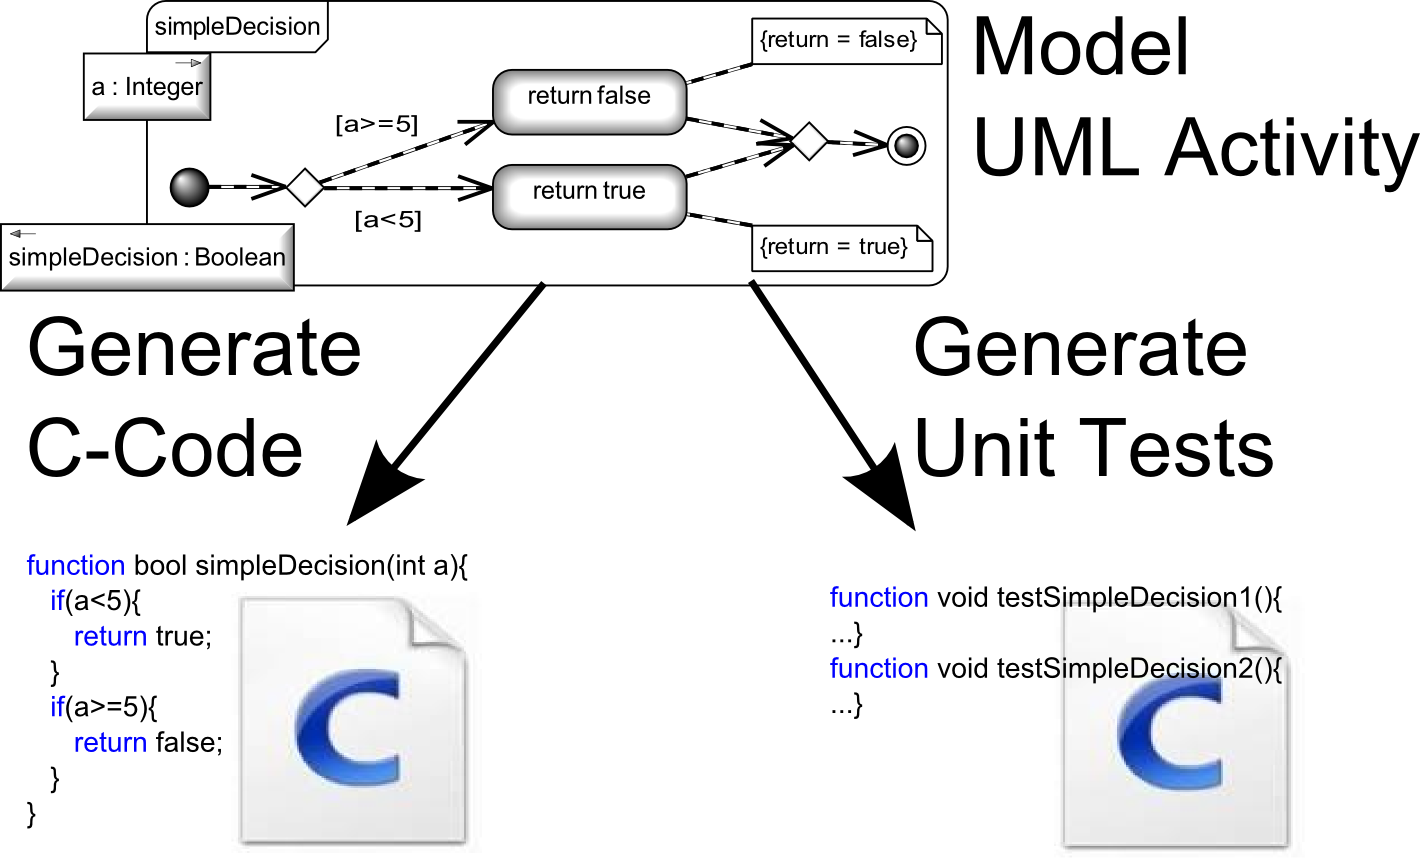
\includegraphics{/pics/Activity2Code+Tests.png}
%\import{{Activity2Code+Tests.pdf_tex}}
\end{frame}

\begin{frame}
\frametitle{Independence of Implementation- and Test-model} 
\begin{itemize} 
\item Artisan automated code synthesis generates C implementation from UML \UMLType{Activity}
\item C Unit tests shall be generated from the same Model
\item Use OCL to specify \emph{localPostCondition} and \emph{guard}s used for Test Generation
\item The structure of the control flow graph is shared between implementation and testmodel
\end{itemize}
\end{frame} 

%\begin{frame}
%%stupid Logo frame
%here you could see some logos of Artisan Airbus and a screen-shot
%\end{frame}


\lecture{Introduction}{intro}
\subsection{Generating Unit Tests from UML Activities}
\begin{frame}
\frametitle{Overall Goals of this Thesis}
\begin{itemize}
\item Develop a tool producing test stimuli from a UML \UMLType{Activity}
\begin{itemize}
\item Integrate seamlessly with existing standard technologies
\item Use mature state-of-the-art constraint solvers
\item Handle non linear mixed integer arithmetic
\item Enable control flow based and boundary based coverage criteria
\item Output JUnit, CPP-Unit test suits
\end{itemize}
\end{itemize}
\end{frame}

\begin{frame}
\frametitle{Generating Unit Tests from a \UMLType{Model}}
\begin{block}{Normalisation}
Map UML/OCL to fully specified intermediate representation
\end{block}
\begin{block}{AMPL Modelling}
Transform into a rigorous mathematical program
\end{block}
\begin{block}{Abstract Test Case Generation}
Select control flow paths according to a test coverage criterion 
\end{block}
\begin{block}{Producing Specific Test Input Values}
Solve mathematical program
\end{block}
\begin{block}{Standard Testing Framework Compatibility}
Output test cases as JUnit or CPP-Unit test suite
\end{block}
\end{frame}

\subsection{Introductory Example}
\begin{frame}[fragile]
\frametitle{Introductory Example}
\begin{columns}
 \column{.4\textwidth} \ 
	\begin{block}{Specifying a Path} 
	\def\svgwidth{\textwidth}
	%\scriptsize
	\import{../FinalPresentation/pics/}{BasicExamples.pdf_tex}
	\end{block} 
\column{.55\textwidth} \ 
	\begin{block}{AMPL} 
		\begin{lstlisting}[basicstyle=\ttfamily\scriptsize,language=ampl]
param l; #Pathlength

# Variables can be Properties, 
# Parameters, Local Variables etc.
var a : integer := 1;
var r in 0..1 := 1;

# Postconditions
set t within {0..l} default {};
s.t. t_post0{i in t} : (r)=(1.0);
set f within {0..l} default {};
s.t. f_post0{i in f} : (r)=(0.0);

# Guards
set d2f within {0..l} default {};
s.t. d2f_g{i in d2f} : (a)>=(6.0);
set d2t within {0..l} default {};
s.t. d2t_g{i in d2t} : (a)<=(5.0);
\end{lstlisting}
	\end{block} 
\end{columns}
\end{frame}

\begin{frame}[fragile]
\frametitle{Introductory Example}
	\begin{block}{Specify Path} 
		\begin{lstlisting}[basicstyle=\ttfamily\small,language=ampl]
param l := 1;
set d2f:= 0; # guard 
set f:= 1; # post condition
		\end{lstlisting}
	\end{block} 
	\begin{block}{Result} 
		\begin{lstlisting}[basicstyle=\ttfamily\small,language=ampl]
Solution determined by presolve.
a = 5
return = 0
		\end{lstlisting}
	\end{block}
\end{frame}


%\begin{frame}
%\frametitle{The Overall Work flow of Generating Unit test from a Model}
%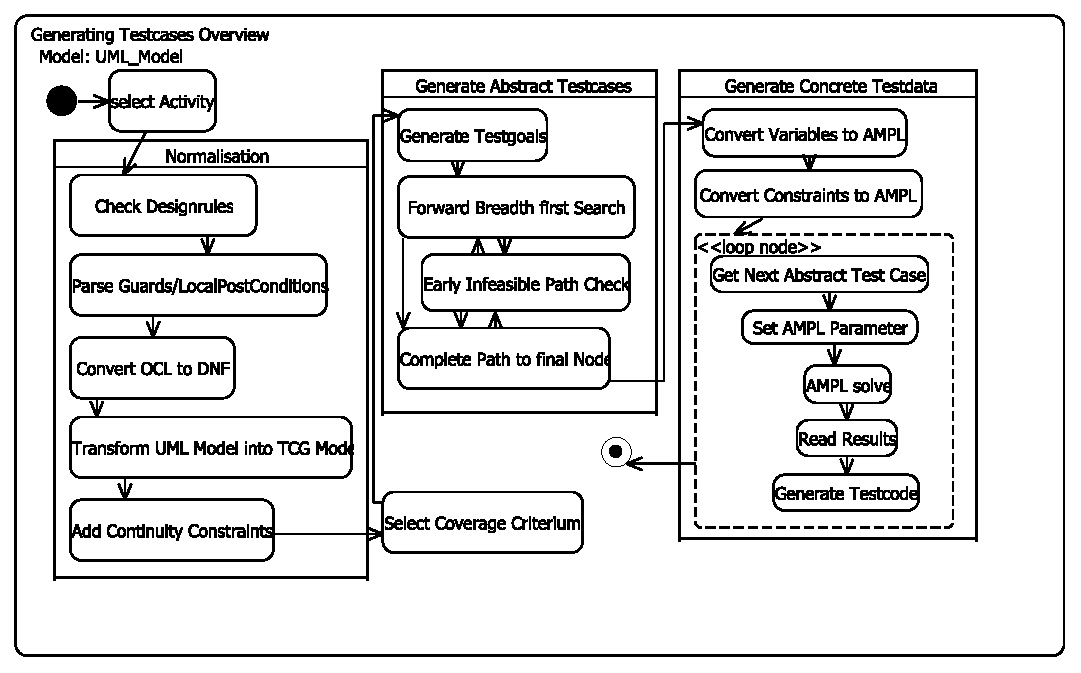
\includegraphics[scale=0.6]{../pics/Workflow.pdf} 
%\end{frame}

%\subsection{Goals of the Tool Development}
%\subsubsection{Normalisation}
%\begin{frame}
%\frametitle{Why do we need Normalisation?}
%\begin{itemize}
%\item Filling in Semantic Variation Points	%Action is mapped to a C Codeblock, Semantic of Parameters
%\item Removal of unnecessary details		%copy only referenced Variables, Remove Namespaces
%\item Removing ambiguous Representations	%OwnedRule instead of LocalPostconditions
%\item Making implicit assumptions explicit 	%else, Continuity Constraints, context Operation
%\end{itemize}
%\end{frame}
%
%\subsubsection{Coverage Criteria and Abstract Testcases}
%\begin{frame}
%\frametitle{Requirements for Abstract Testcase generation}
%\begin{itemize}
%\item Produces an effective suite of relevant test cases
%\item Supports a variety of Coverage Criteria
%\item Do not get stuck in loops or combinatorial explosion
%\item eliminate infeasible paths as early as possible
%\end{itemize}
%\end{frame}
%
%\begin{frame}
%\frametitle{Definition of Abstract Test Cases}
%%an abstract testcase is one specific Path and potentially Additional constraints specifiying valueassignments of subexpressions.
%\end{frame}
%
%\subsubsection{Constraint Solving for Specific Test Stimuli}
%\begin{frame}
%\frametitle{Wish List for Generating Specific Values}
%\begin{itemize}
%\item Support for a large subset of OCL specification
%\begin{itemize}
%\item Arithmetic constraints (linear and non-linear)
%\item Set expressions and operations
%\item Object type variables
%\end{itemize}
%\item Efficient algorithms for variety of constraint systems
%\item Interchangeability of Constraint Solvers
%\end{itemize}
%\end{frame}


\section{Generating Test Cases Step by Step}
\subsection{Activity Test Case Graph}

\begin{frame}
\frametitle{Activity Test Case Graph}
\begin{itemize}
\item An activity contains \emph{nodes} and \emph{edges} and \emph{variables}
\item A node can be supplied with multiple \emph{localPostconditions}
\item An edge has exactly one \emph{guard}
\item Variables
\begin{itemize}
\item Can be basic variables (\UMLType{Integer}, \UMLType{Boolean}, \UMLType{Float}) or compound variables (\UMLType{Collection}, \UMLType{Object})
\item Basic variables can be changeable (\UMLType{Data Store}, \UMLType{Property}) or fixed (\UMLType{Parameter})
\item Basic variables are referenced by expressions
\end{itemize}
\item \emph{Activity Test Case Graph} is a refinement of the more general \emph{Abstract Test Case Graph} meta model
\end{itemize}
\end{frame}

\begin{frame}
\frametitle{The Activity Test Case Graph Class Model}
	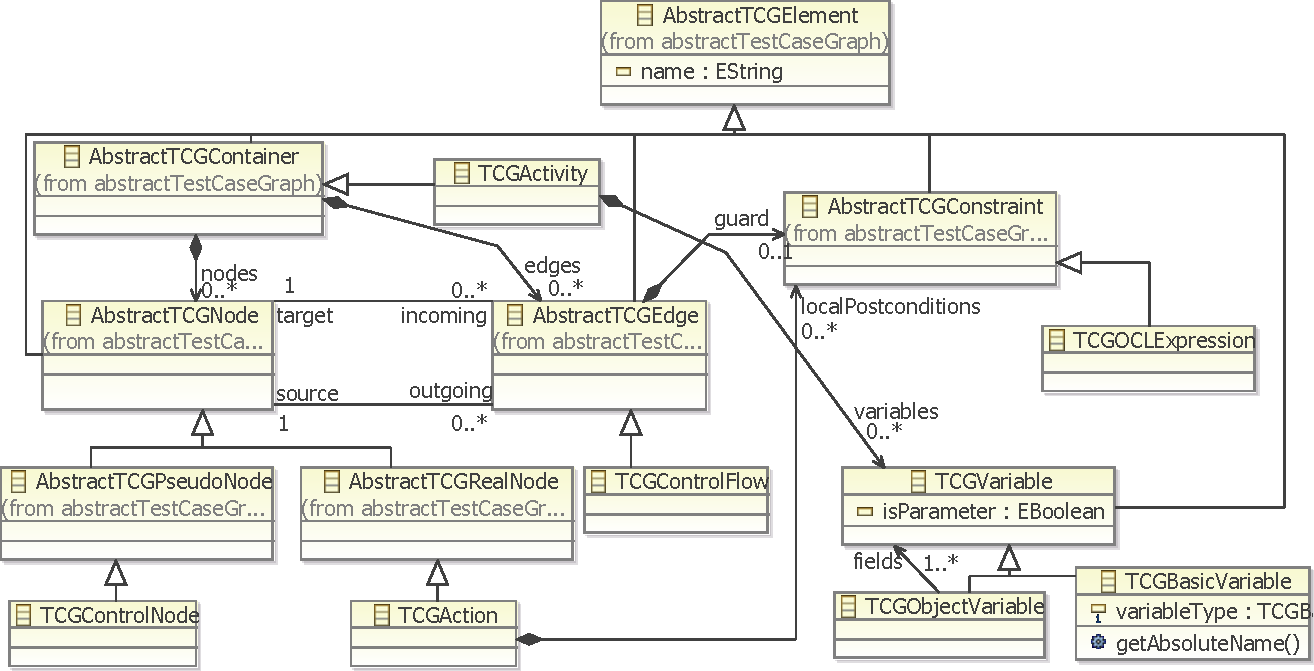
\includegraphics[width=\textwidth]{pics/completeMetamodelforSlideshowN.pdf}
\end{frame}

%\begin{frame}
%\frametitle{Parsing OCL Constraints}
%\begin{itemize}
%\item Each UML tool supports different ways you could use to embed OCL Constraints
%\item Many UML tools do not offer proper OCL editing support
%\item Eclipse UML/OCL can parse Invariants for NameSpaces and PostConditions for Operations
%\item Guards are parsed as Invariant, LocalPostconditons as Postconditions
%\item An Operation specifying the Activity is necessary to provide the parser with a valid context
%\item Local Variables need to be added manually to the context
%\end{itemize}
%\end{frame}

\begin{frame}
\frametitle{More Normalisations}
\begin{itemize}
\item Successfully parsed \UMLType{Constraint}s are added to the \emph{Activity Test Case Graph} model
\item Variables relevant to the expressions are included in the \emph{Activity Test Case Graph} model
\item => there is only one single name space in the \emph{Activity Test Case Graph} Model
\item Add additional \emph{localPostconditions} stating, that for each node unreferenced variables should not change
\item Until now only basic variables (integer, float, boolean) are handled
\end{itemize}
\end{frame}

\subsection{Generating AMPL Model}
\begin{frame}
\frametitle[test]{Generating the AMPL Model}
\begin{itemize}
\item Model to Text Transformation from \emph{Activity Test Case Graph} to AMPL model language
\begin{itemize}
\item Constant Variables become a single Variable
\item Variables become an array with one field per Action on the execution path
\item \emph{guard}s and \emph{localPostconditions} become constraints
\end{itemize} 
\item When a boundary value is demanded a linear objective function can be added to the AMPL model
\item The exact control flow path for which input data should be found is specified in the AMPL data
\end{itemize}
\begin{block}{The Resulting Problem}
In general non linear, mixed integer constraints and a simple, linear objective function
\end{block}
\end{frame}

\subsection{About the Solvers}
\begin{frame}[fragile]
\frametitle{Solvers that work with AMPL\cite{AMPL} }
\ctable[
cap=solvers,
width = \textwidth,
]{cc}{}{ \FL
Solver & Problem Types
\ML
CPLEX \cite{cplex}& linear, mixed-integer, quadratic \NN
ILOGCP \cite{ILOGCP}& SAT with CPLEX for arithmetic\NN
LP-SOLVE\cite{lpsolve} & linear \NN
COUENNE\cite{COUENNE} & non linear, mixed-integer, global search \NN
GECODE\cite{gecode}& combinatorial (SAT-based eager approach) \NN
MINOS\cite{minos} & local non linear \LL
}
\end{frame}

\begin{frame}
\frametitle{Problems with Solvers still to Solve}
\begin{itemize}
\item Most non linear solvers need a starting point
\begin{itemize}
\item Let the user provide starting points
\item Try multiple times with random starting points
\item Find feasible solution with globally converging solver and then use optimizer to find boundary value
\end{itemize}
\item Logical constraints are not supported by most solvers
\begin{itemize}
\item Transform logical constraints into arithmetic constraints
\item Transform \emph{Activity Test Case Graph} to eliminate logical constraints
\item Use Satisfiability Modulo Theories (SMT) Solver
\end{itemize}
\end{itemize}
\end{frame}

\begin{frame}
\frametitle{Examples}
\begin{block}{Strict Inequality}
Logical: $x<5$ \hspace{1cm} Arithmetic: $x<=5-\epsilon$;
\end{block}
\begin{block}{AND}
Logical: $(a<=5) and (a>=0)$ \hspace{1cm} Arithmetic: $a<=5$; $a>=0$
\end{block}
\begin{block}{OR}
Logical: $(a<=5) or (a>=10)$ \\Arithmetic: $z1*a>=z1*5$; $ z2*a>=z2*10$; $z1+z2>=1$;
\end{block}
\begin{block}{Graph Transformation}
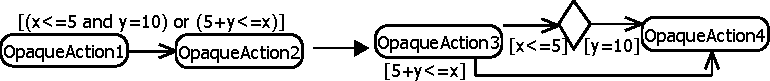
\includegraphics[width=\textwidth]{pics/transformLocigGuards.pdf}
\end{block}
\end{frame}

\subsection{Finding Control Flow Paths}

\begin{frame}
\frametitle{How to produce Efficient Test Suits}
%add ParTeG Logo here
\begin{itemize}
\item ParTeG\cite{ParTeG}
\begin{itemize}
\item Implements coverage criteria to generate test goals
\item A backward search algorithm tries to find feasible paths fulfilling a test goal
\item The test goal manager checks which test goals are already fulfilled
\item The general architecture of the test goal management can be adapted to \emph{Activity Test Case Graph} models
\end{itemize}
\item Currently we use a bounded depth first search to find control flow paths
\end{itemize}
\end{frame}


\section{Outlook} 

\begin{frame}
\frametitle{Potential further explorations}
\begin{itemize}
\item Support variety of coverage criteria
\begin{itemize}
\item Adapt ParTeG's test goal management and coverage criteria implementation
\end{itemize}
\item Combine path search with early infeasible path elimination
\begin{itemize}
\item Improve solver interaction
\item Possibly improve overall solving time
\end{itemize}
\item Support more UML/OCL features
\begin{itemize}
\item How to model arbitrary data types and references
\item How to handle call hierarchy
\item Which variables to fix when invariants and postconditions interfere
\end{itemize}
\item Verify the UML to AMPL transformation
\begin{itemize}
\item Create test suite from case study 
\item Formal verification
\end{itemize}
\item Support other algebraic modelling systems costing less than 4000\$ 
\end{itemize}
\end{frame}

\section*{Appendix}
\begin{frame}
\begin{block}{Thank you!}
\begin{center}
\Huge{Questions?}
\end{center}
\end{block}
\end{frame}

\frametitle{Bibliography}
\bibliographystyle{IEEEtran}
%\bibliographystyle{plain}
\bibliography{../Thesis/bibtex}


\end{document}
